\section{事例重建}\label{sec:evt_reco}
重建是指将探测器各个子系统的着火点或者能量沉积的低级信息转换成与对撞中产生的粒子相关的高级信息的过程。
ATLAS中的重建是一个由集中式软件框架中的众多算法执行的复杂的多步骤过程\cite{Calafiura:2005zz},其最终输出是用于各种物理分析的物理对象(也简称为“对象”),包括电子,光子,$\mu$子,喷注和强子$\tau$候选者,以及MET。 下面将概述重建这些物理对象的基本步骤,更多地关注与本文中$hh$和$t\bar{t}H$搜索相关的对象。

\subsection{径迹和能量簇射}
重建的基本输入是径迹和能量簇射。

径迹是由带电粒子经过ID或者MS造成的一系列着火点构成的。
径迹重建\cite{Cornelissen:1020106}的初始种子是探测器(Pixel和SCT)中的三个空间着火点。
它们通过组合迭代算法形成径迹候选者,随后拟合到螺旋轨迹\cite{Cornelissen_2008},同时需要考虑材料效应,能量损失和多次散射以及磁场非均匀性。
然后通过根据每个候选者的属性(例如重合测量数量和拟合质量)对轨迹进行排序来解决模糊性。 最后轨迹被外推到TRT,并且在完整轨迹上执行新的拟合。
然后基于重建径迹使用专业算法\cite{Piacquadio_2008}决定每个束团对撞的顶点候选者,以及可用于识别重味喷注的次级顶点。

$\mu$子候选者的径迹通过连接ID中的轨迹与MS重建的轨迹得到。MS轨道搜索算法\cite{Benekos_2008}首先搜索精密室中的命中模式,以在每层中形成直线轨道段;
然后通过片段种子组合算法找到$\mu$子MS径迹候选者,并且根据全局$\chi^{2}$拟合得分接受或拒绝与每个候选者相关联的着火点。

来自量能器的能量簇射是ATLAS中粒子重建的另一个基本输入。 
穿过量能器的电子,光子和强子与活性材料相互作用而失去能量,并在纵向和横向上留下几个量能器单元的信号。 来自电子和光子的簇射主要包含在EM量能器中,而强子通常在HCal中产生簇射。
簇射算法\cite{Lampl:1099735}将着火单元组合在一起,根据粒子种类使用不同的逻辑,并将每个簇射内的总沉积能量相加,同时确定位置。根据进入的粒子类型(电子和光子,或强子射流),校准能量以补偿簇射外或者死区的能量沉积。

结合径迹和量能器簇射信息最终可以鉴别物理对象,图~\ref{fig:particle_id_patterns}显示ATLAS不同粒子的径迹和能量沉积模式。
\begin{figure}
\centering
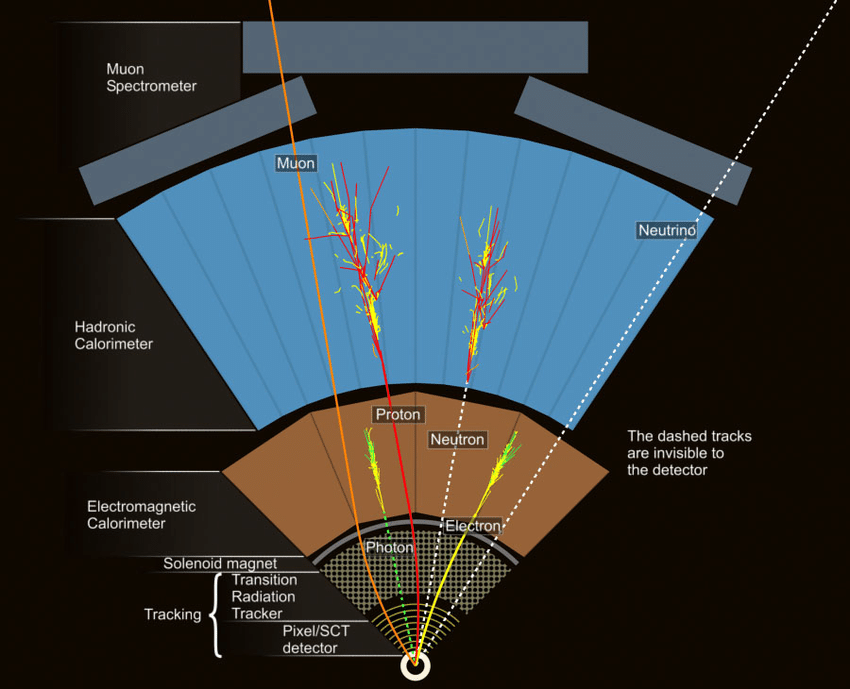
\includegraphics[width=0.75\textwidth]{fig/particle_ID_patterns.png}
\caption{不同粒子在ATLAS探测器($r-\phi$平面)的径迹和能量沉积情况。}
\label{fig:particle_id_patterns}
\end{figure}

\subsection{电子}
电子和光子在EM量能器中有非常相似的特征。两个对象之间的主要区别在于电子也会在ID中留下径迹。ATLAS有许多基于光子末态的物理分析,因为它们具有非常好的能量分辨率。然而,本文分析并没有涉及光子,所以不述光子鉴别,光子重建的细节可以在参考文献\cite{ATLAS-CONF-2012-123}中找到。

对于电子,其簇射通过滑动窗口算法进行\cite{Lampl:1099735},即在一定范围内搜索使3$\times$5单元窗口(单元大小为0.025$\times$0.025,$\eta\times\phi$)内具有最大沉积能量并将其作为初始簇射种子,
即塔(tower\footnote{
%A tower in the EM calorimeter represents the set of cells contained in a 0.025$\times$0.025 ($\eta,\phi$)unit spanning longitudinally over the 3(4) calorimeter layers.
代表一系列着火单元,形状如塔。
}),
电子径迹重建如前面讲述,但考虑到电子通过ID时因韧致辐射造成的稍大的能量损失,会使用特定的模式识别和拟合假设。
使用高斯和滤波器(Gaussian Sum Filter)\cite{ATLAS-CONF-2012-047}重新拟合在$(\eta,\phi)$平面与EM簇射松散匹配的电子轨迹,以更好地考虑致辐射过程中的非线性。 然后在更严格的条件下匹配重新拟合后的轨迹与簇射,例如要求一定的最小硅着火点数以及在最内层Pixel中存在着火点以排除在ID中转换的光子。 电子能量由EM簇射给出,其最终校准基于蒙特卡罗模拟\cite{Aad2014-cali},而$\eta$和$\phi$坐标由相应的轨道参数给出。

电子重建仅针对$\abseta<2.47$和$\et >$7 GeV,对于$\pt>$15 GeV电子,重建效率大概在97\%到99\%。重建效率的测量基于$Z\rightarrow ee$和$J/\Psi\rightarrow ee$事例\cite{ATLAS-CONF-2016-024}\textbf{Update?},其结果如图\ref{fig:ele_reco_eff}所示,数据和模拟样本中的效率差别在$\mathcal{O}(1)\%$水平,而且在实际分析中此相对差别会作为修正因子考虑到MC中。
\begin{figure}[h]
\begin{center}
\begin{subfigure}[b]{0.45\textwidth}
\centering
      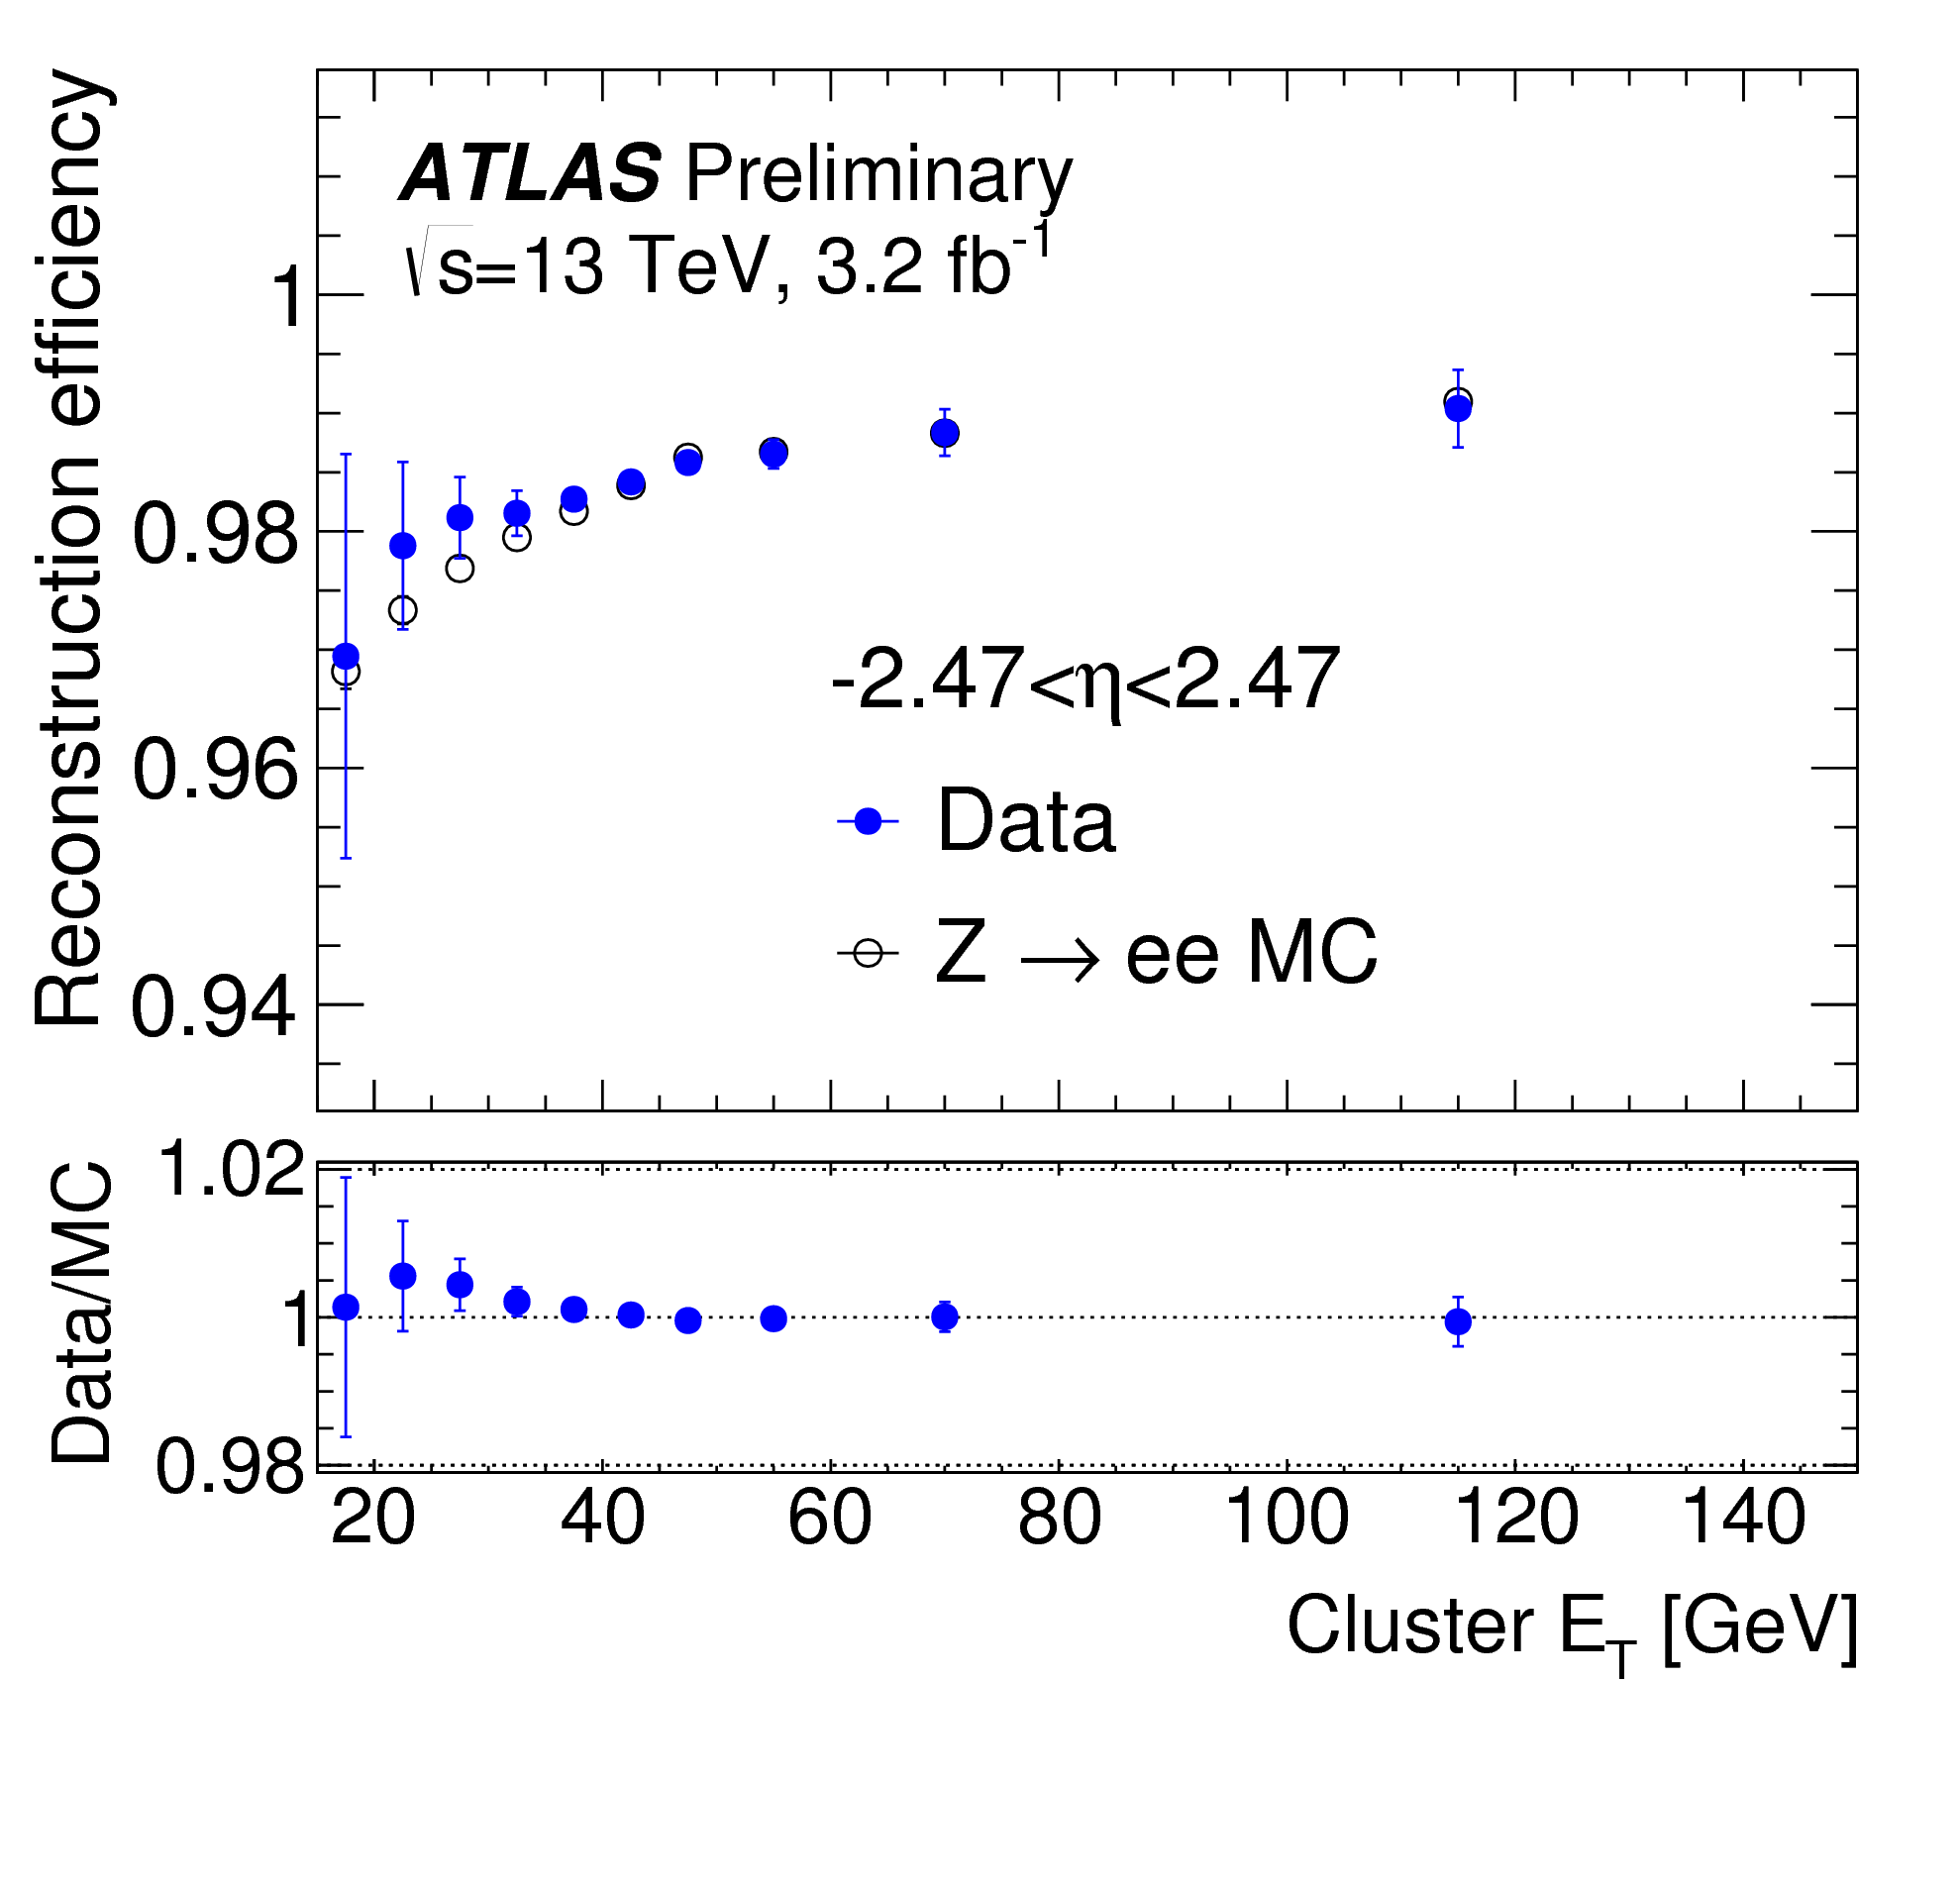
\includegraphics[width=\textwidth]{fig/ele_reco_eff.png}
     \caption{}
      \label{fig:ele_reco_pt_eff}
  \end{subfigure}
 \begin{subfigure}[b]{0.45\textwidth}
 \centering
      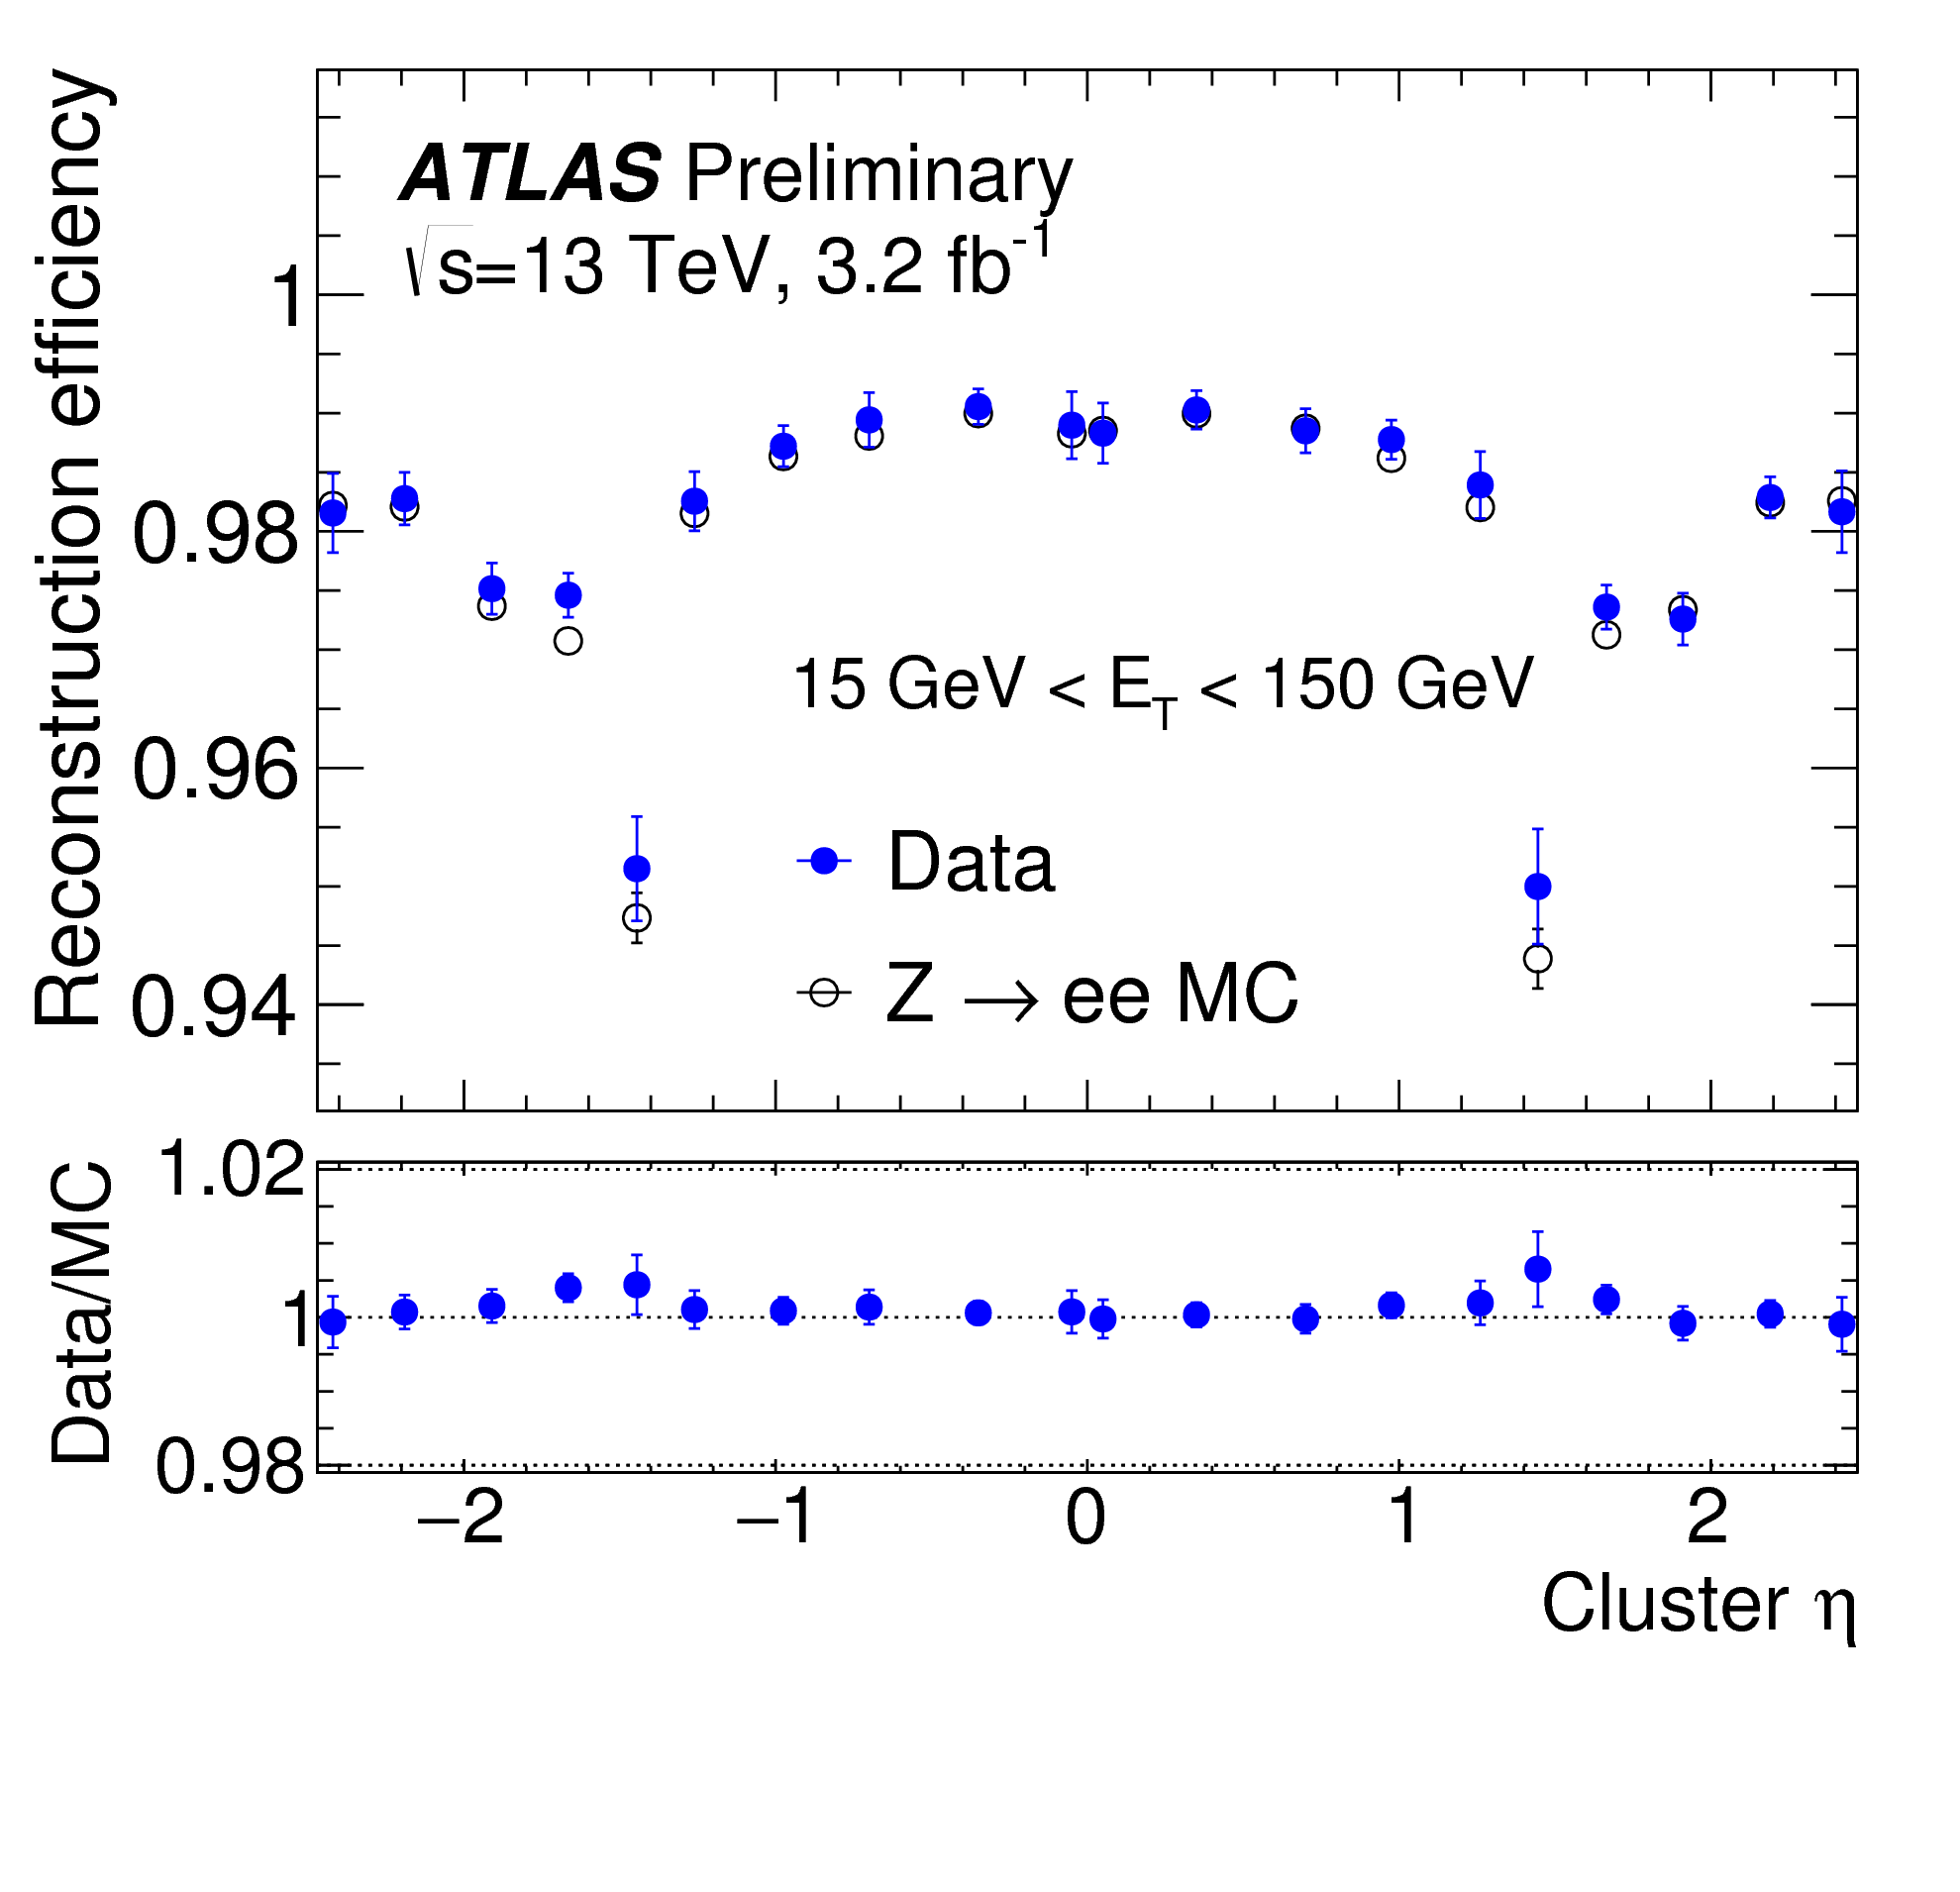
\includegraphics[width=\textwidth]{fig/ele_reco_eta_eff.png}
      \caption{}
      \label{fig:ele_reco_eta_eff}
  \end{subfigure}
\caption{2105年数据与$Z\rightarrow ee$~MC中的电子重建效率随簇射\et (a)和簇射$\eta$ (b)分布情况\cite{ATLAS-CONF-2016-024}。} 
 \label{fig:ele_reco_eff}
\end{center}
\end{figure}

电子鉴别(\texttt{ID})通过基于似然函数多变量判别式\cite{ATLAS-CONF-2016-024}进行。算法的输入变量包括量能器簇射形状,基于TRT穿越辐射的似然概率和轨道-簇射匹配相关量,以及轨迹的测量总数和IBL中的测量数量和韧致辐射变量。
基于不同鉴别效率,定义三个电子鉴别工作点,分别命名为\texttt{Loose}, \texttt{Medium}和\texttt{Tight}。对于\et =25 GeV真实电子而言,它们的鉴别效率在78-90\%,而相应的本底误判率为0.3-0.8\%。
图\ref{fig:ele_id_eff_pileup}展示各个工作点随pileup数的变化情况,基本上其效率比较稳定。
\begin{figure}
\centering
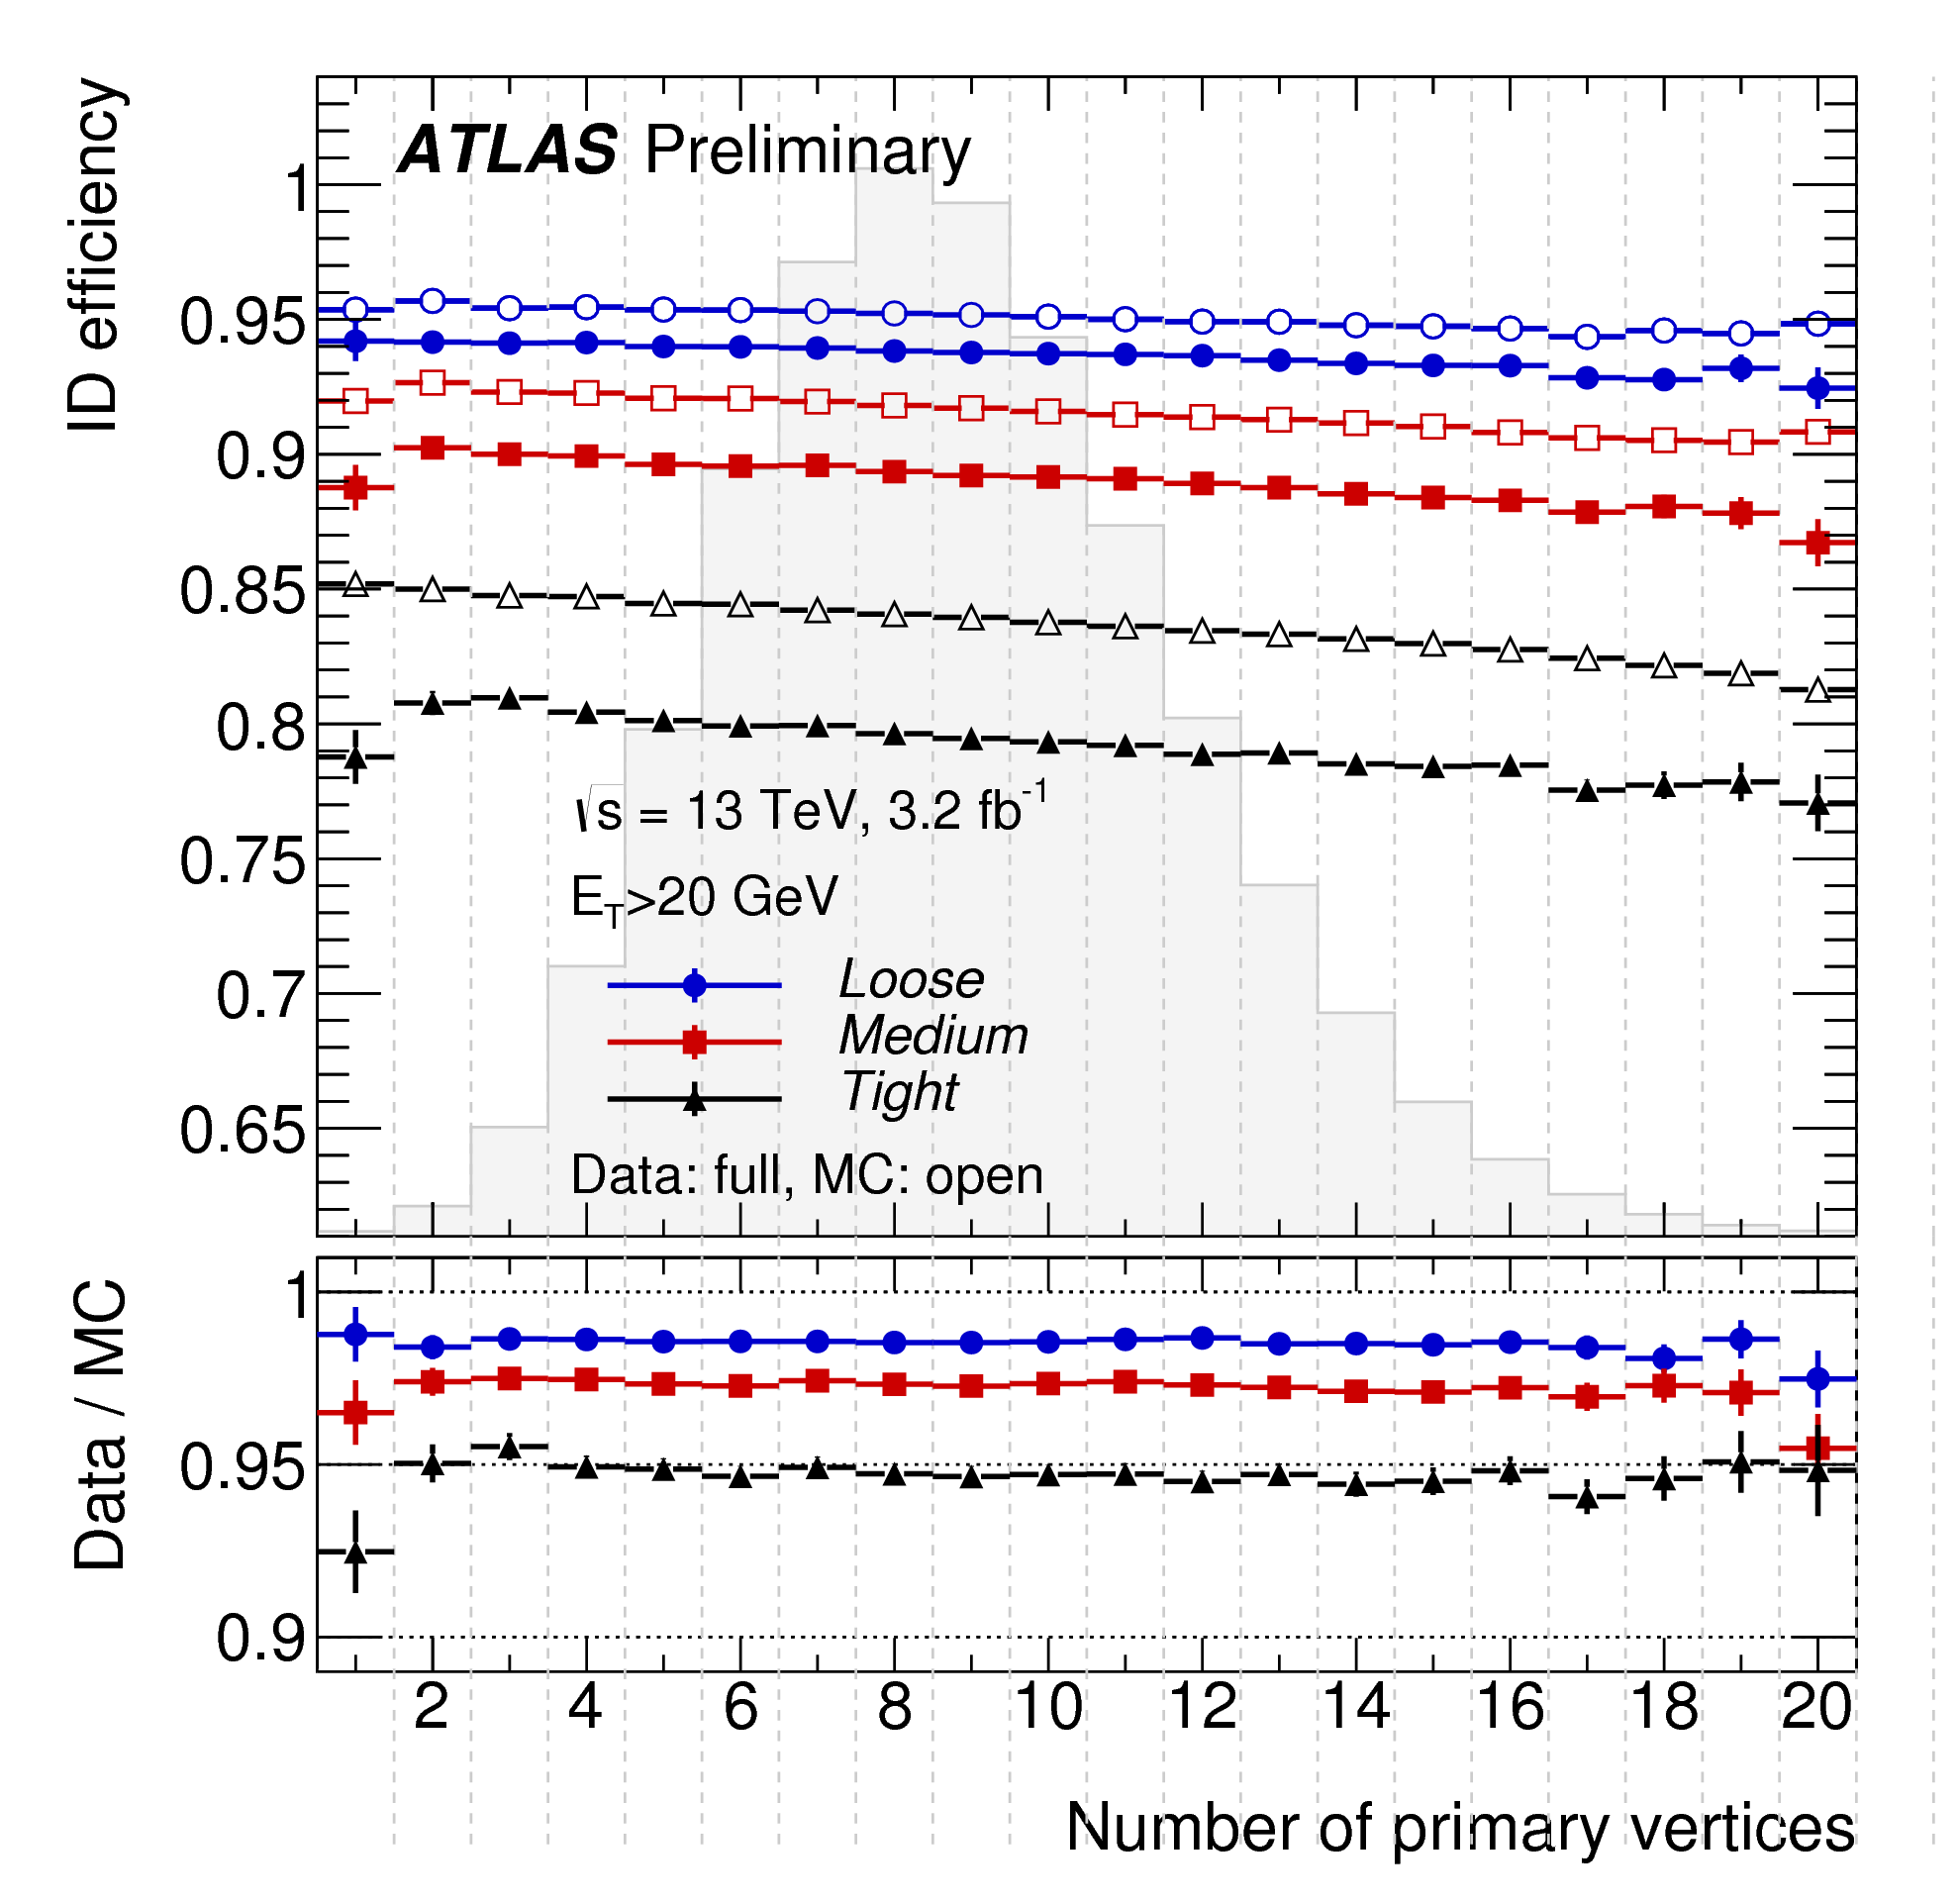
\includegraphics[width=0.65\textwidth]{fig/ele_id_eff_pileup.png}
\caption{2015年数据和$Z\rightarrow ee$~MC在不同工作点的鉴别效率随顶点数分布情况\cite{ATLAS-CONF-2016-024},背景中的灰色直方图为顶点数的分布情况。}
\label{fig:ele_id_eff_pileup}
\end{figure}

$Z\rightarrow ee$和$J/\Psi\rightarrow ee$事例也用来测量触发效率\cite{ATLAS-CONF-2016-024}。图\ref{fig:ele_trigger_eff}展示2015年使用的单电子触发器\footnote{\texttt{HLT\_e24\_lhmedium\_L1EM20VH}}效率随\et 和$\eta$ 的变化,在$\et>$27 GeV时,触发效率
可达95\%,数据与MC之间的差别在5\%以内。最大的偏差发生在24 GeV附近,这是因为在L1阶段,数据与MC使用了不同的阈值,MC会根据这些差别进行修正。
\begin{figure}[h]
\begin{center}
\begin{subfigure}[b]{0.45\textwidth}
\centering
      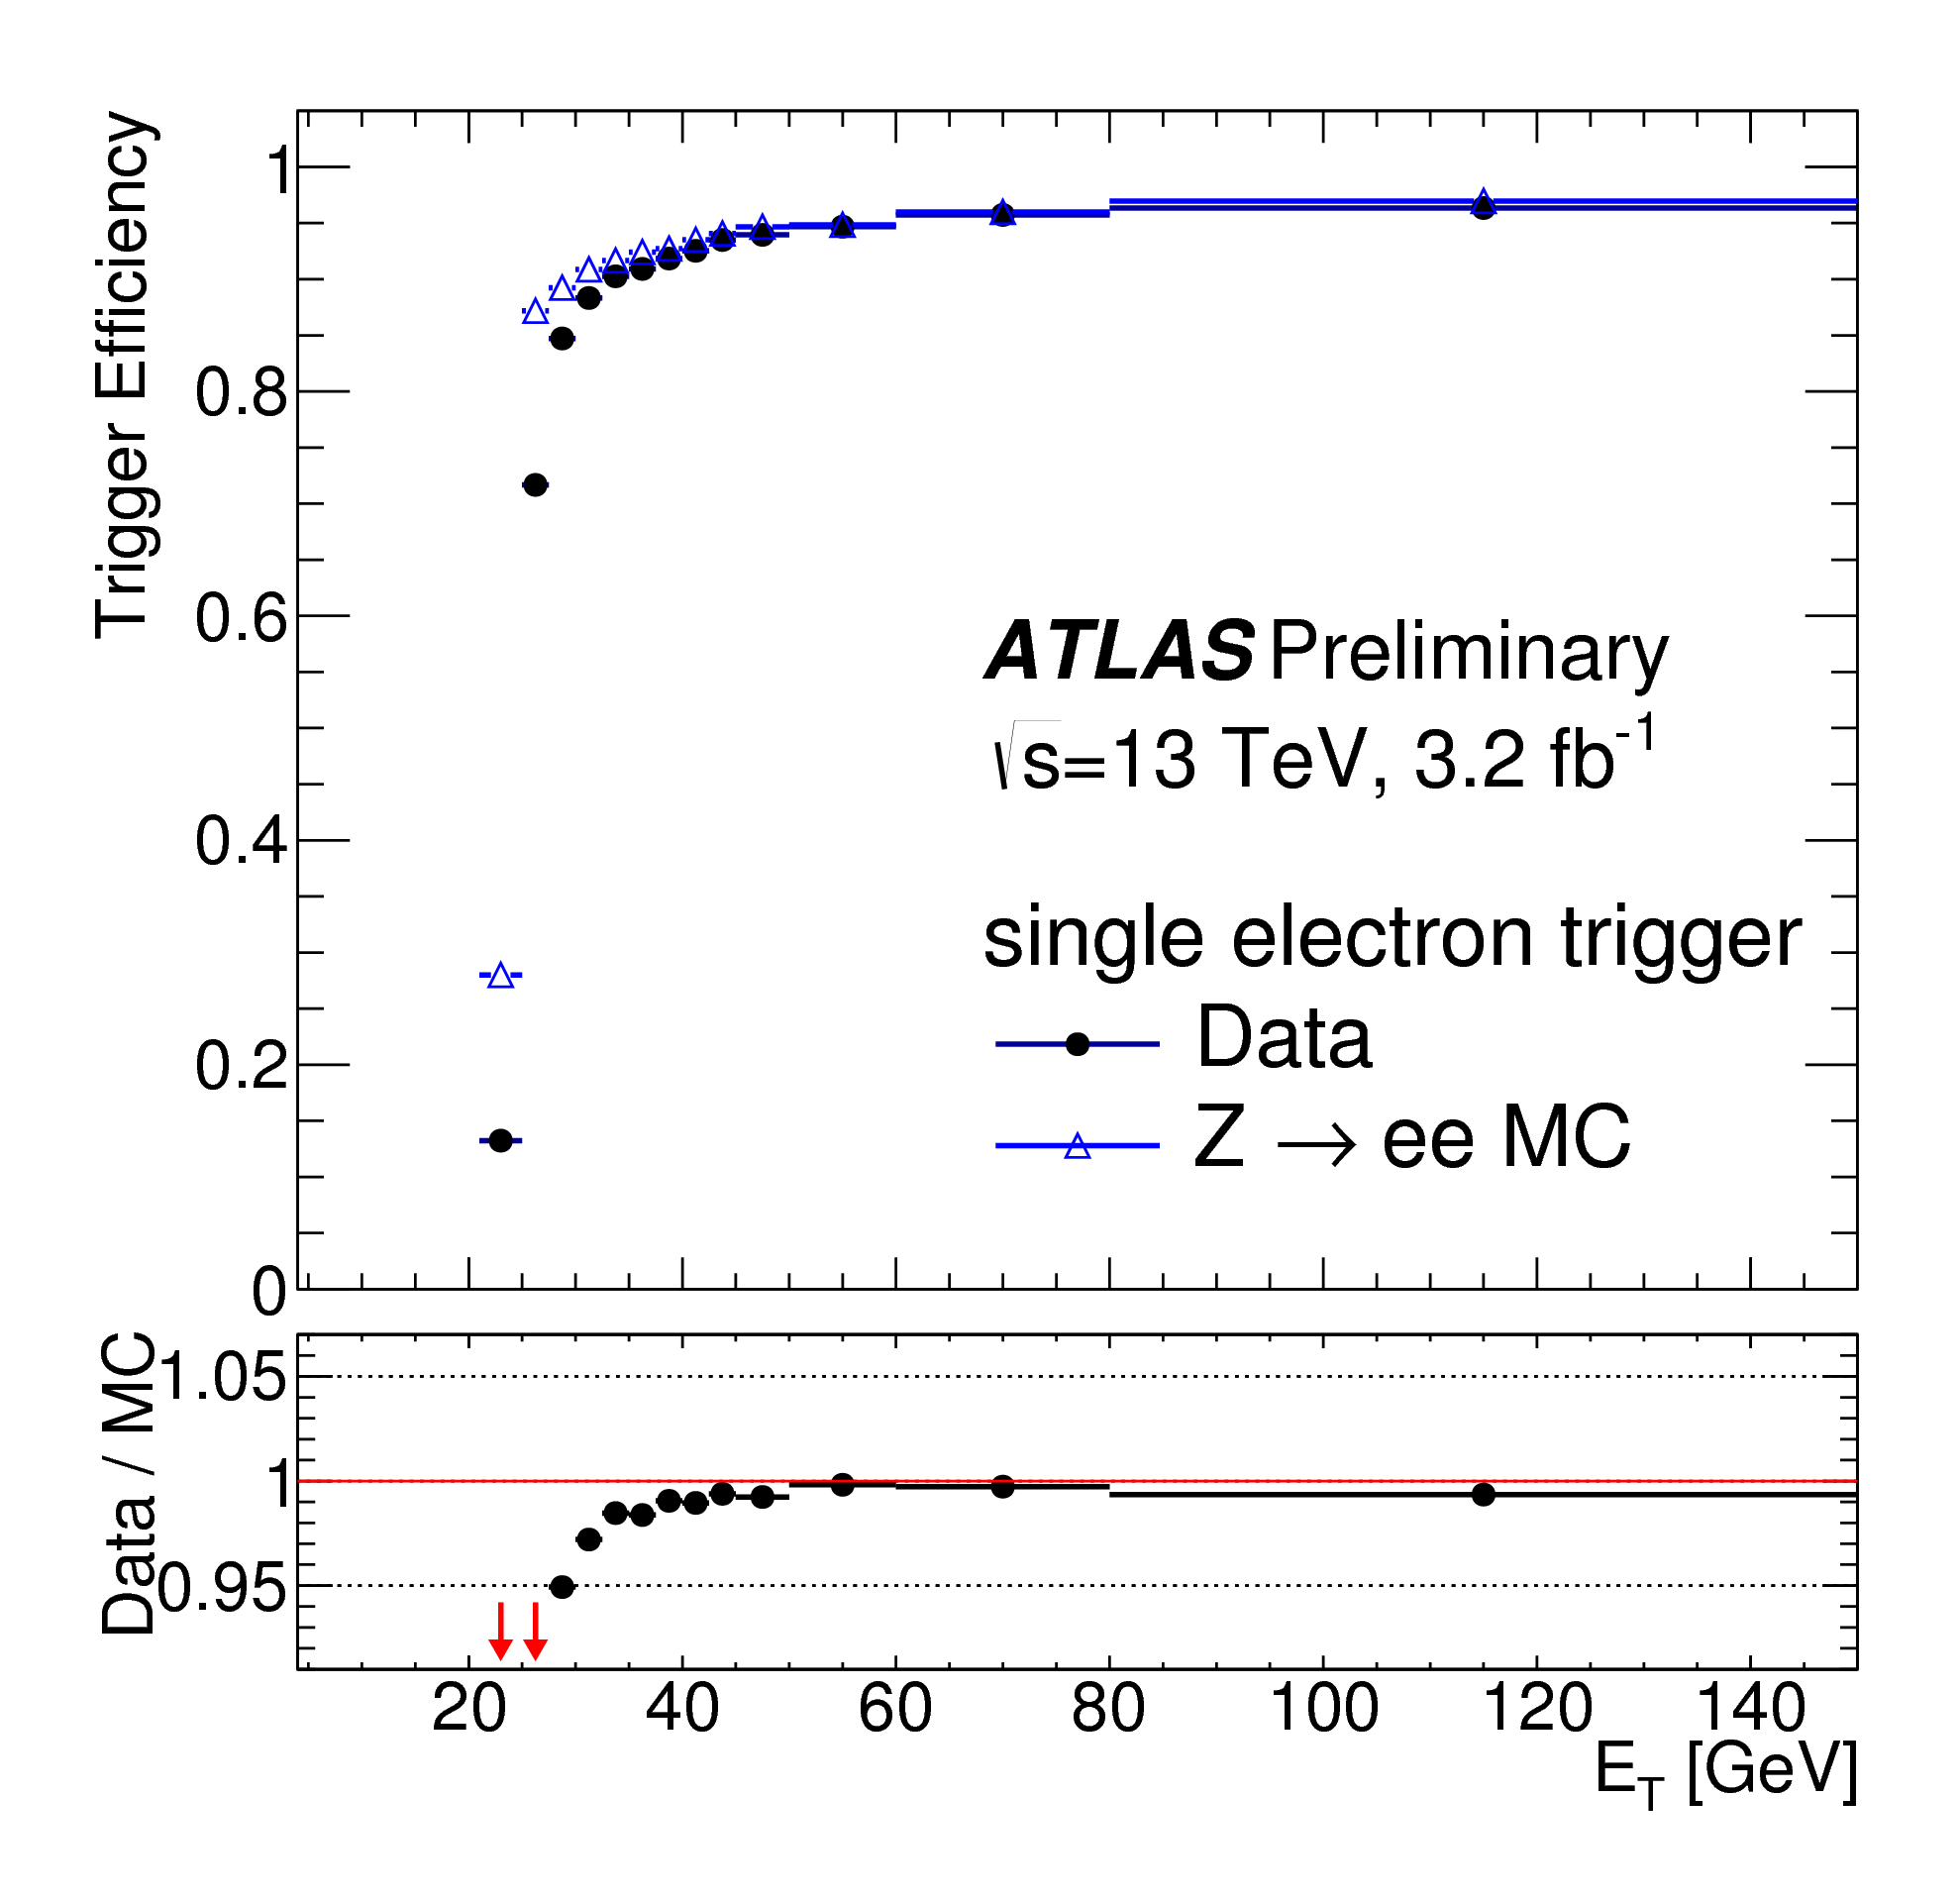
\includegraphics[width=\textwidth]{fig/ele_trigger_eff_et.png}
     \caption{}
      \label{fig:ele_trigger_et_eff}
  \end{subfigure}
 \begin{subfigure}[b]{0.45\textwidth}
 \centering
      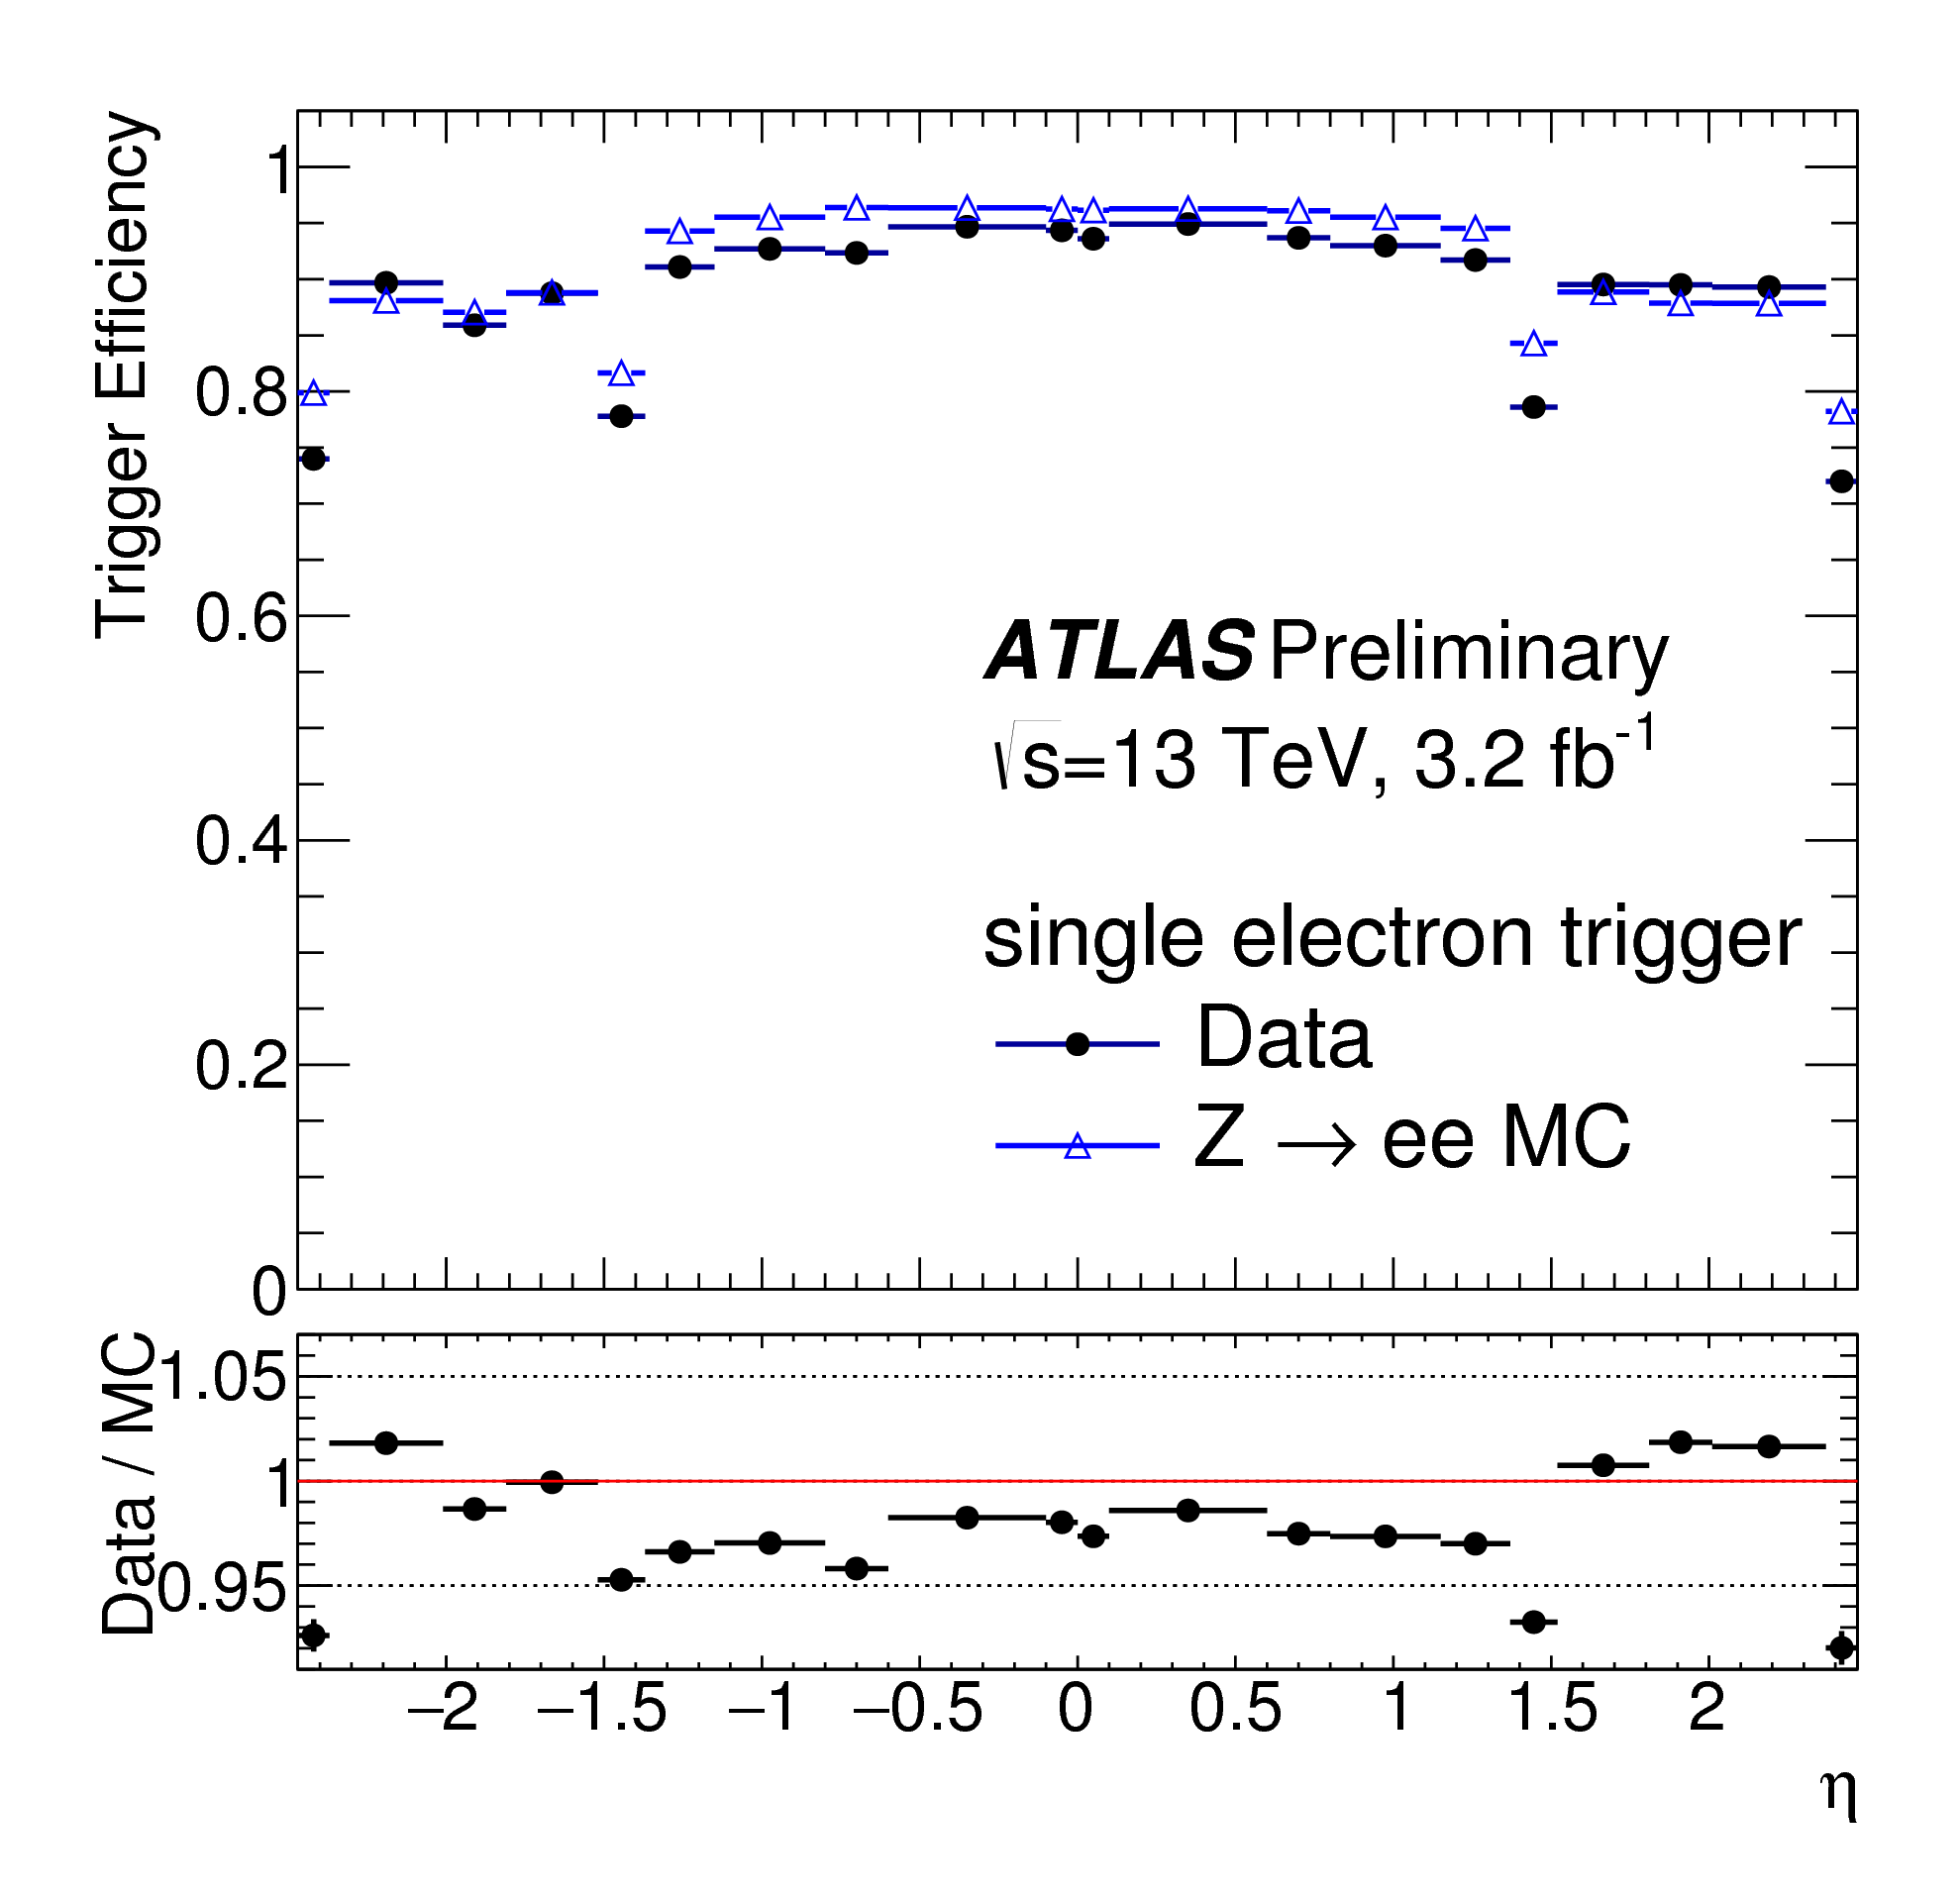
\includegraphics[width=\textwidth]{fig/ele_trigger_eff_eta.png}
      \caption{}
      \label{fig:ele_trigger_eta_eff}
  \end{subfigure}
\caption{2015年电子和$Z\rightarrow ee$~MC的单电子触发效率随\et~(a)和$\eta$~(b)的分布情况\cite{ATLAS-CONF-2016-024}。} 
 \label{fig:ele_trigger_eff}
\end{center}
\end{figure}

\subsection{$\mu$子}
$\mu$子重建联合利用ID和MS的径迹,以及量能器信息,它有四类:
\begin{itemize}
 \item Combined muons (CB). 这些$\mu$子通过同时拟合ID和MS的着火点得到,在拟合过程中,MS着火点可以被添加或者移除已改善拟合质量。
 \item Segment tagged muons (ST). 这类$\mu$子代表当完整ID轨迹仅与MDT或CSC中的一个轨道段(segment)匹配时的情况,这要么是因为\pt 低或者因为它们穿过MS接收度低的区域。
 \item Calorimeter tagged muons (CT). 来自电弱衰变的高动量$\mu$子在穿过量能器时仅沉积很少的能量,与最小的电离损失相当。当ID轨迹与一个这样的簇射匹配时,则定义为CT~$\mu$子候选者。 
 这些$\mu$子是假的概率较高,但可以在MS探测器件较少的$\abseta<0.1$区找回一些。
 \item Extrapolated muons (ME). 为了处理ID未覆盖的前向区$2.5<\abseta<2.7$,可以仅重建MS的轨迹,然后考虑在量能器内的能量损失后外推回初级顶点。
\end{itemize}
不同类别的$\mu$子重叠消除之后,才定义物理分析可用的对象粒子。值得指出的是,$\mu$子重建可到4 GeV。与电子类似,有三个$\mu$子质量工作点:\texttt{Loose}, \texttt{Medium}和\texttt{Tight}。
\texttt{Tight}$\mu$子仅包括CB类,并且有额外的径迹质量要求以压低不是初级顶点来的$\mu$子;\texttt{Medium}~$\mu$子也包括$\abseta>2.5$的ME类,但是要求至少存在要个MS径迹segment;
\texttt{Loose}$\mu$子也包括ST和CT类。

$\mu$子重建效率的评估与电子类似,利用$Z\rightarrow \mu\mu$和$J/\Psi\rightarrow \mu\mu$事例\cite{Aad2016-mu2016}。对于\texttt{Loose}类和\texttt{Medium}类,重建效率为98\%,而对于\texttt{Tight}类,平均为95\%。图\ref{fig:muon_reco_eff}总结2016年$\mu$子重建效率情况,可以看到,数据与MC的差别在几个百分点,主要集中在MDT对齐稍差的桶部区。
\begin{figure}[h]
\begin{center}
\begin{subfigure}[b]{0.45\textwidth}
\centering
      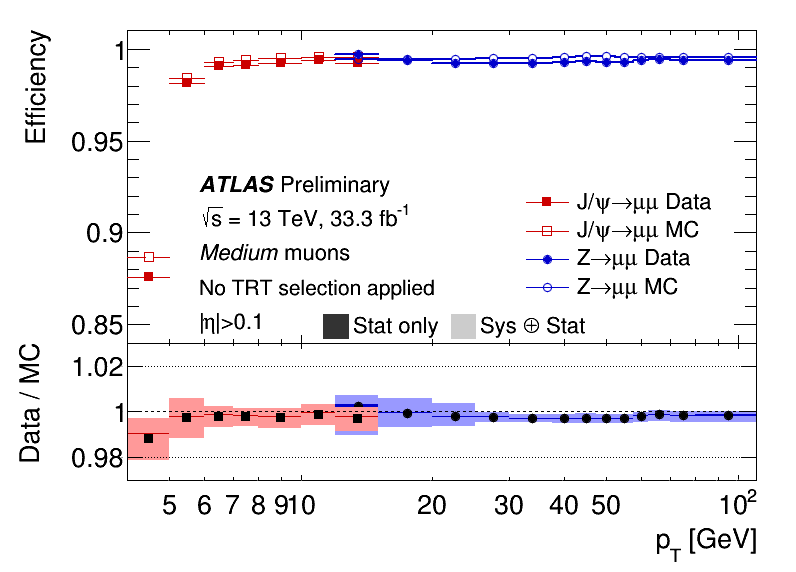
\includegraphics[width=\textwidth]{fig/muon_reco_eff_pt.png}
     \caption{}
      \label{fig:muon_reco_eff_pt}
  \end{subfigure}
 \begin{subfigure}[b]{0.45\textwidth}
 \centering
      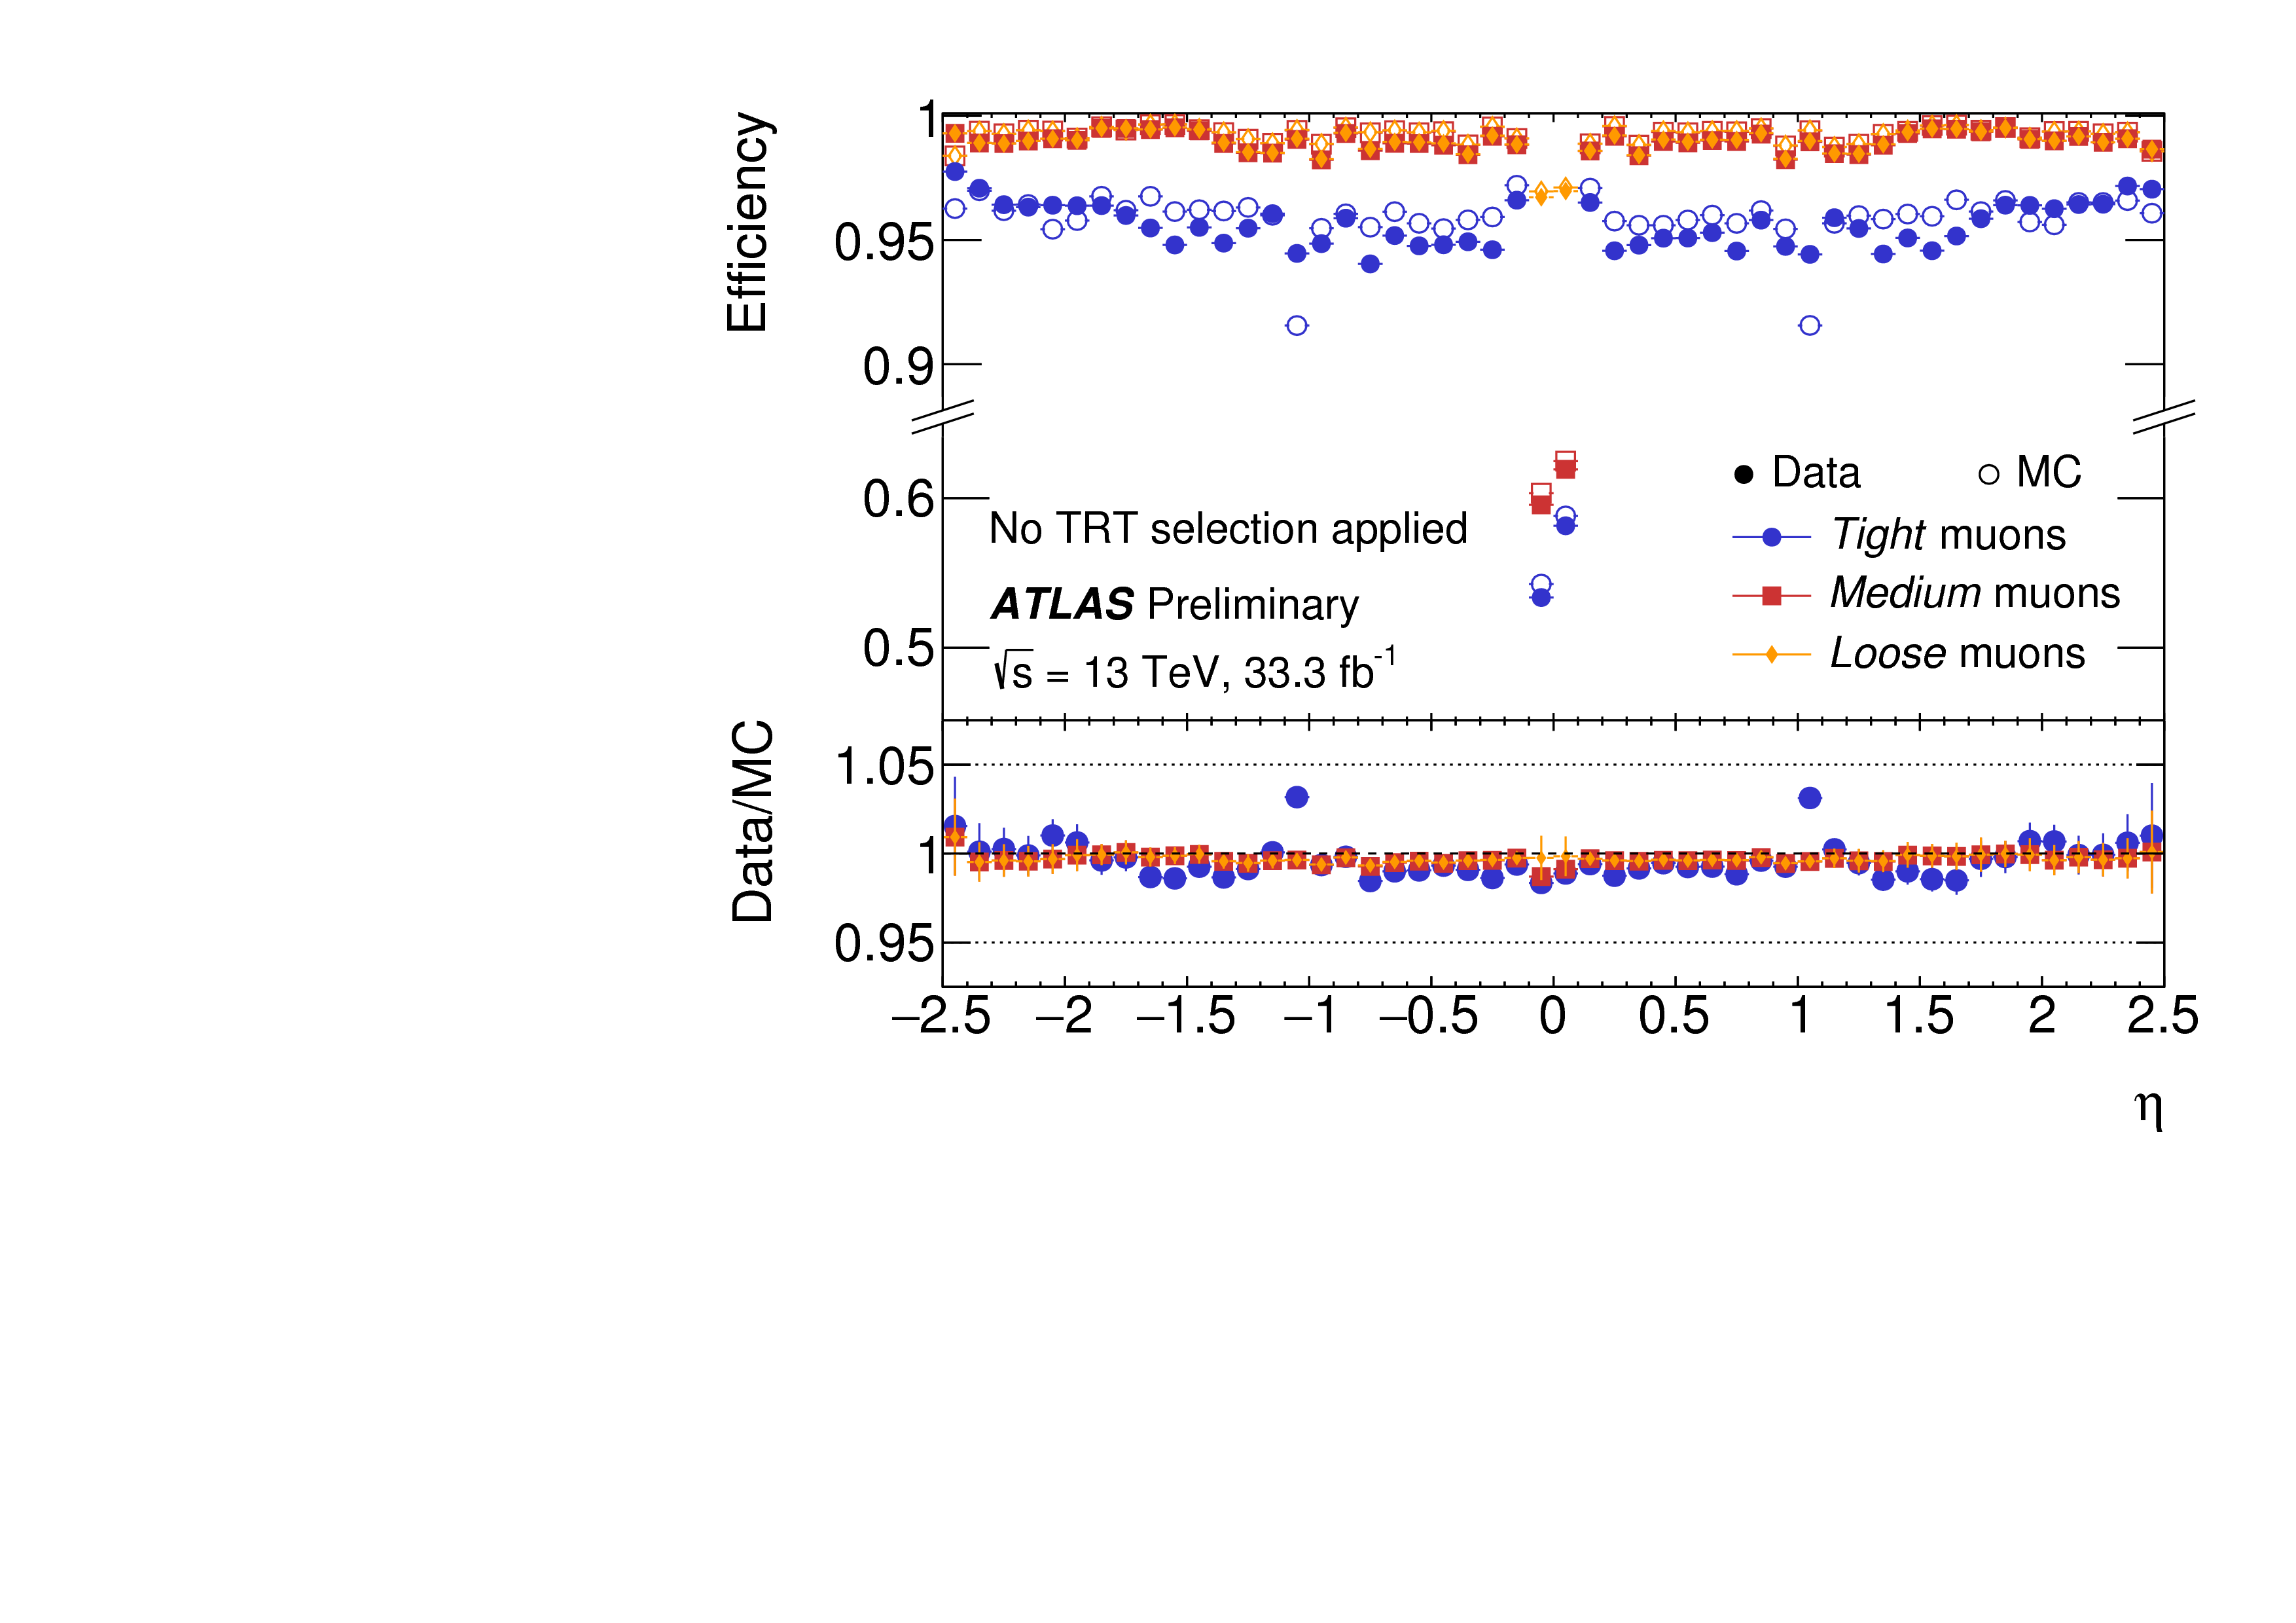
\includegraphics[width=\textwidth]{fig/muon_reco_eff_eta.png}
      \caption{}
      \label{fig:muon_reco_eff_eta}
  \end{subfigure}
\caption{2015+2016年数据与$Z\rightarrow \mu\mu$,  $J/\Psi\rightarrow \mu\mu$~MC中的$\mu$子重建效率随\pT~(a)和$\eta$~(b)分布情况,(b)中$\abseta<0.1$区间\texttt{Loose}~$\mu$子效率
的回升是因为使用calorimeter-tagged的$\mu$子定义。} 
 \label{fig:muon_reco_eff}
\end{center}
\end{figure}

$\mu$子触发效率\cite{Muon-trigger-results}表现估计与电子类似。图~\ref{fig:muon_trigger_eff}展示L1 MU20触发器的效率,这类触发要求MS中至少存在一个$\pt>$20 GeV的$\mu$子候选者。
L1桶部触发效率大约为70\%,而在前向区为90\%,这是因为RPC比TGC更少的几何接收度。然而对于通过L1的$\mu$子,HLT触发效率可达100\%。数据与MC之间的触发效率在几个百分比水平。
\begin{figure}[h]
\begin{center}
\begin{subfigure}[b]{0.45\textwidth}
\centering
      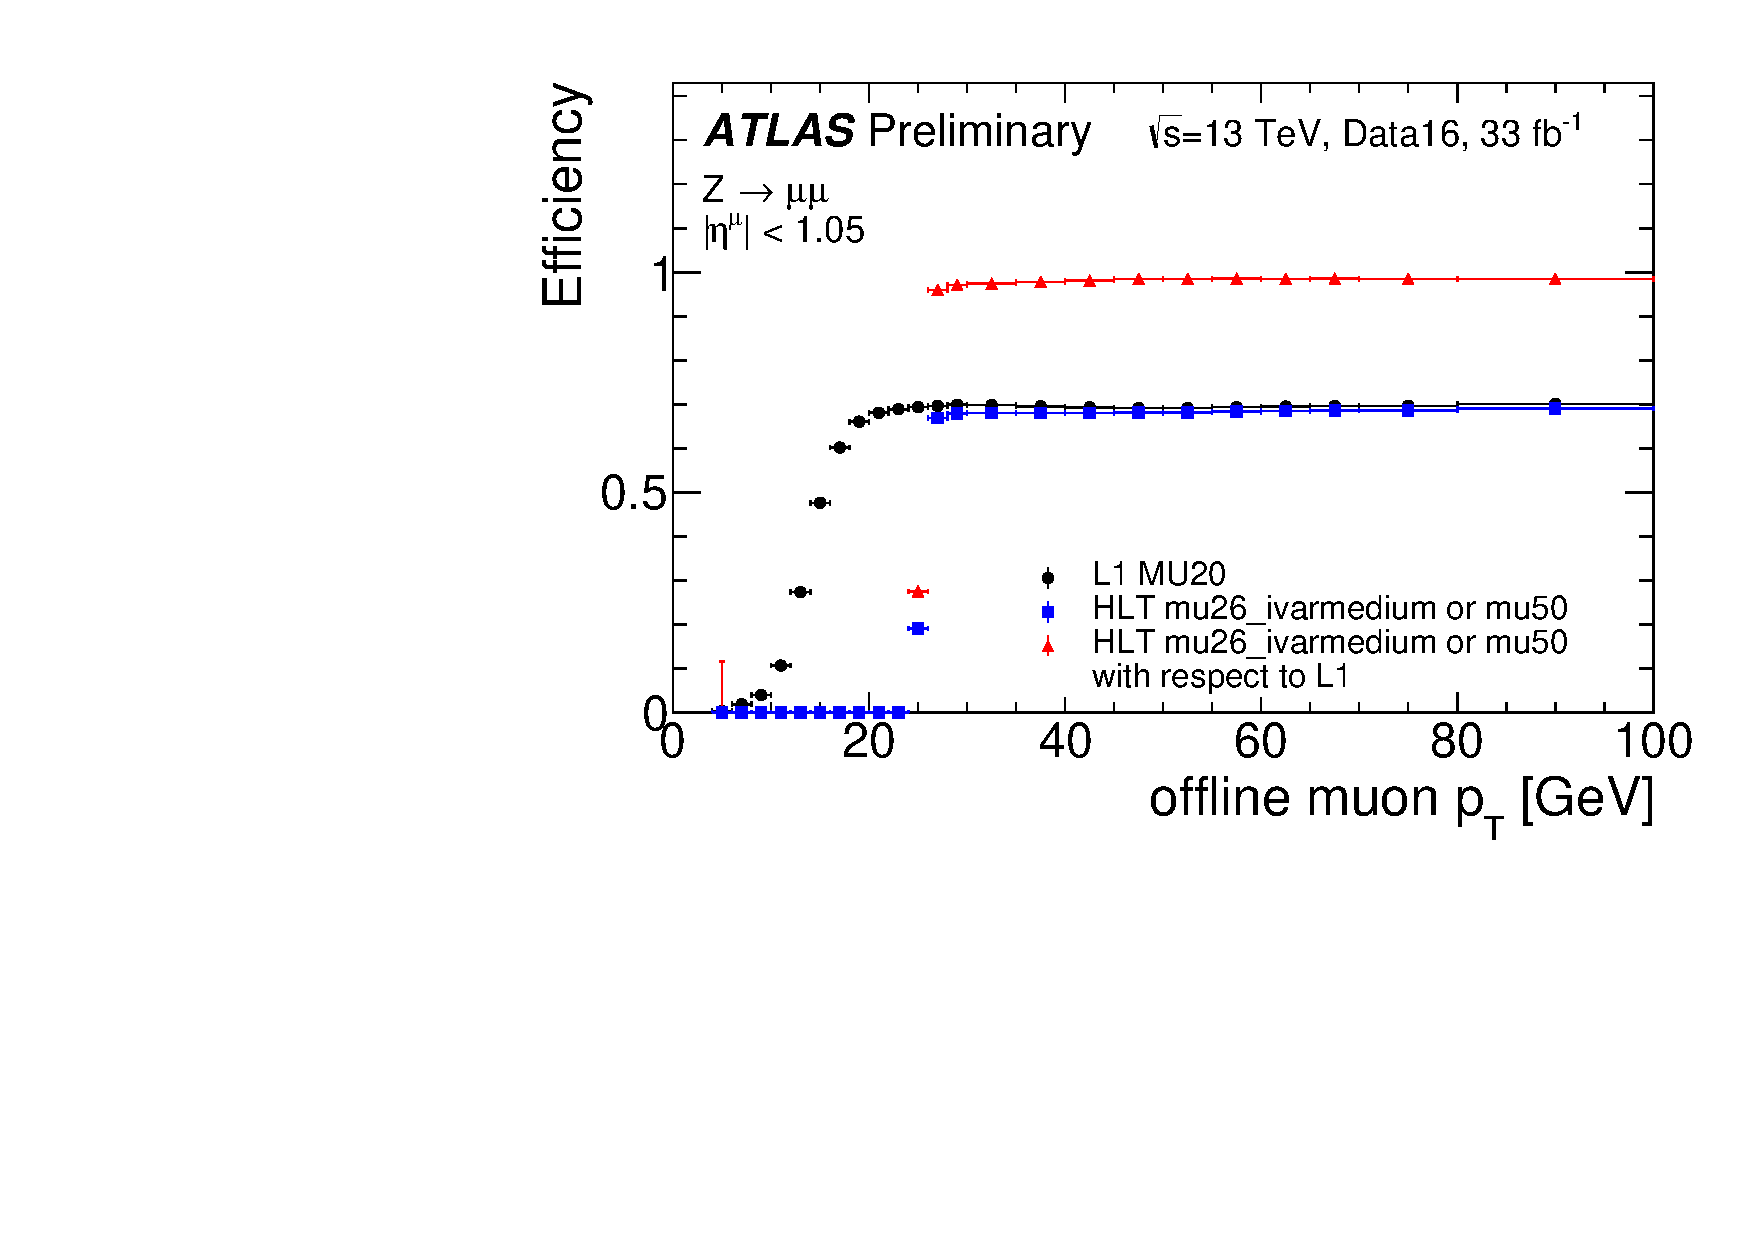
\includegraphics[width=0.7\textwidth,angle=-90]{fig/HLT_mu26_ivarmedium_OR_HLT_mu50_Medium_IsoFixedCutTightTrackOnly_barrel_probe_pt_eff.pdf}
     \caption{}
      \label{fig:muon_trigger_eff_pt_barrel}
  \end{subfigure}
 \begin{subfigure}[b]{0.45\textwidth}
 \centering
      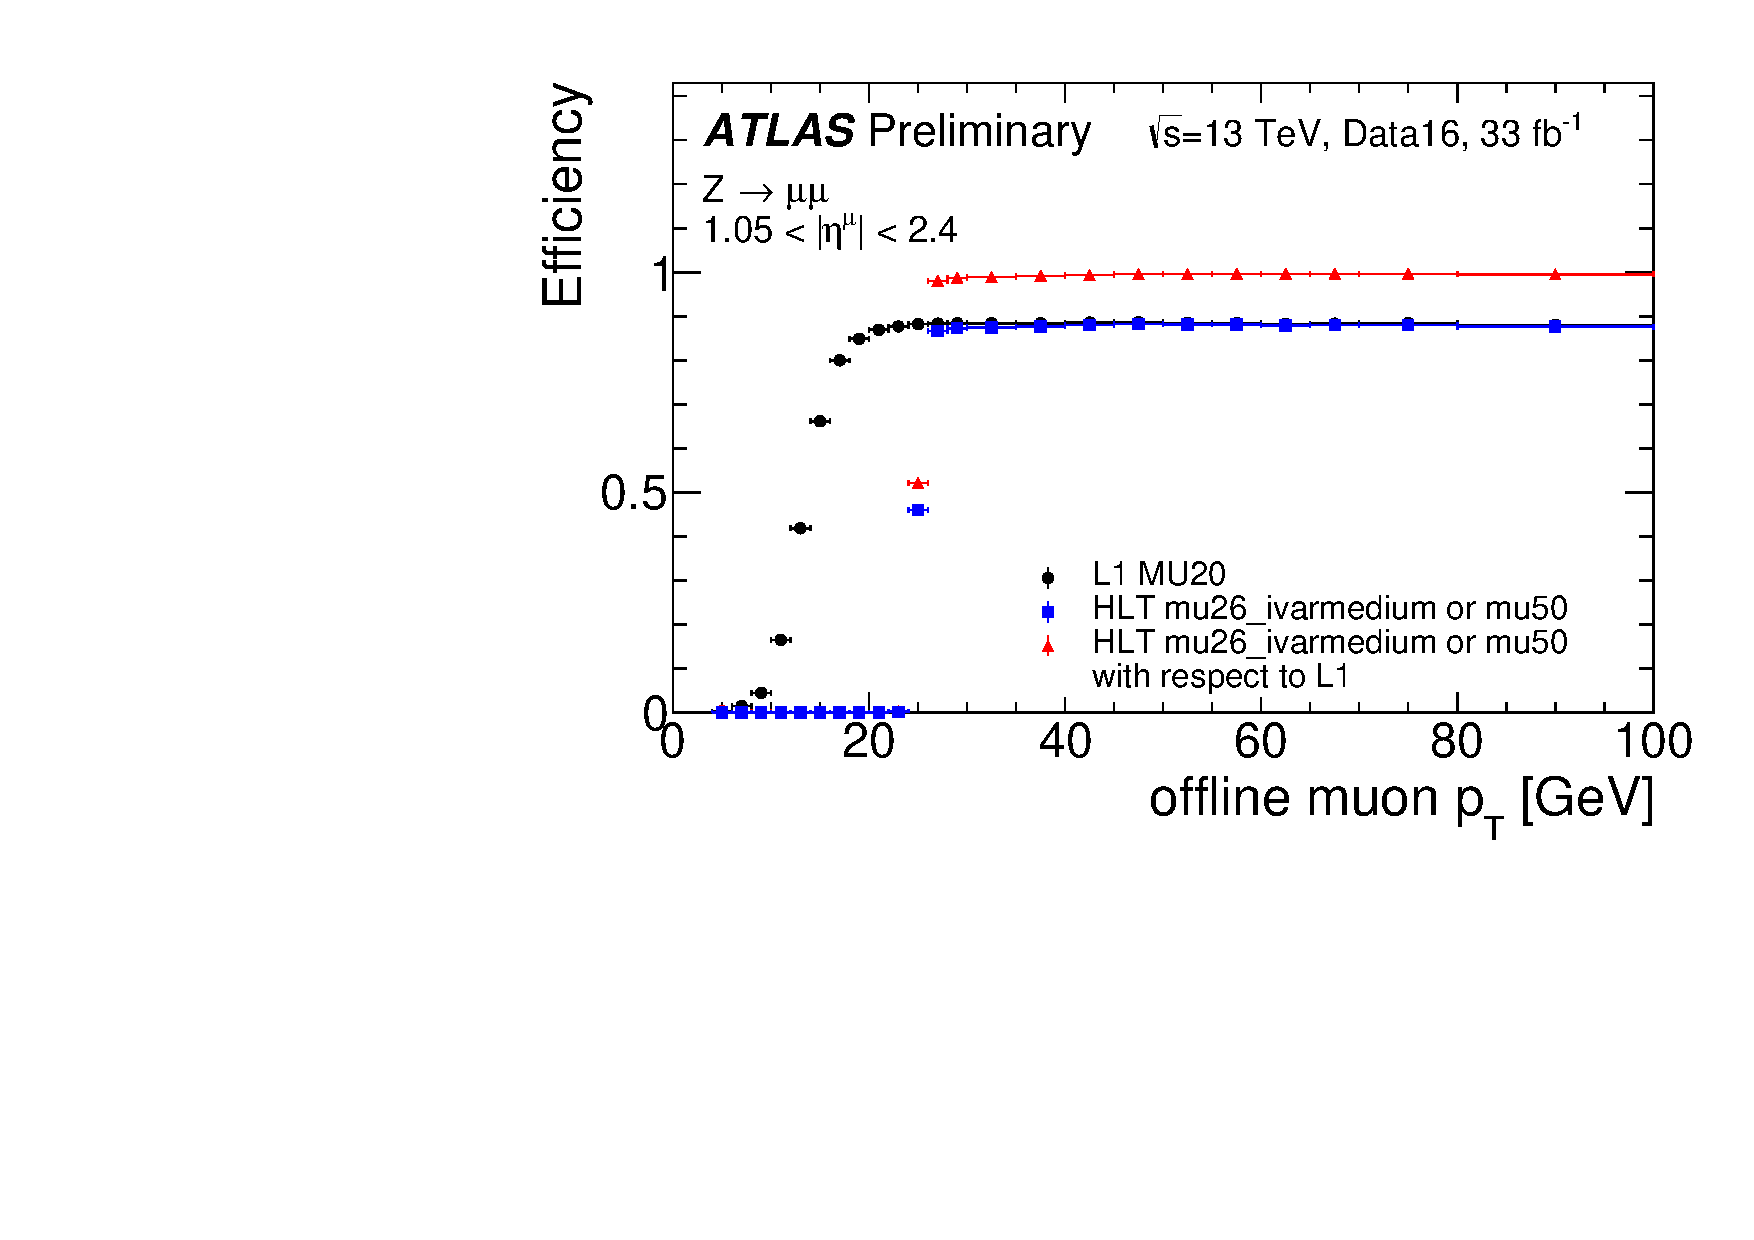
\includegraphics[width=0.7\textwidth,angle=-90]{fig/HLT_mu26_ivarmedium_OR_HLT_mu50_Medium_IsoFixedCutTightTrackOnly_endcap_probe_pt_eff.pdf}
      \caption{}
      \label{fig:muon_trigger_eff_pt_endcap}
  \end{subfigure}
\caption{2015+2016年数据中L1 MU20 seed的触发效率随\pT~分布\cite{Muon-trigger-results},HLT的在线筛选对$\mu$子有一定的isolation要求。}
%The online selection at HLT includes a requirement of low activity around the muon candidate (isolation).} 
 \label{fig:muon_trigger_eff}
\end{center}
\end{figure}
MC中$\mu$子动量大小和分辨率会根据对撞数据校准\cite{Aad2016-mu2016},其相对分辨率在1.7\%与2.9\%之间,在校准之后,对于大部分\abseta 区域数据与MC的分辨率相差在5\%以内。

\subsection{喷注}\label{subsec:jet_reco}
硬散射过程中的末态夸克和胶子(也包括初态辐射)会通过虚胶子的微扰辐射产生部分子簇射,当簇射能量传递下降到典型的强子尺度$\Lambda_{\text{QCD}}\approx$20 GeV时,%?
QCD微扰论不再适用,强子化过程开始,即形成无色荷的束缚态。

从探测器角度看,强子化的结果是一束相互比较靠近的强子,被称为喷注(jet),显然,喷注的能量和方向是与初始部分子直接相关的。
ATLAS喷注重建算法的输入是相邻的着火单元簇射(topoclusters)\cite{Aad:2016upy}。
%在本文物理分析中使用的喷注是由在电磁能量标度(EM)下校准的topoclusters构建的,
%它正确地测量了量能器中电磁簇射的沉积能量\cite{ATLAS-CONF-2013-004}。
本文使用的喷注是由在电磁能量标度(EM)下刻度的topoclusters构建的。

本文使用的喷注是利用\antikt 算法\cite{Cacciari:2008gp}在$\Delta R$=0.4范围基于topoclusters构建的,其($\pt>$25 GeV)能量大小和分辨最终通过仿真的技术校准到真实部分子能量,而且在data-driven中得到证实\cite{TheATLAScollaboration:2015soq,TheATLAScollaboration:2013pia}。

$\pt<$60 GeV, $\abseta<$2.4的喷注有一定概率的来自\pileup ,一个称为喷注顶点标记(JVT)\cite{ATLAS:2014cva}的算法通过关联喷注径迹与顶点可以压低\pileup 影响。在$t\bar{t}H$分析对
该算法的应用中,每个喷注的平均关联效率为92\%。JVT的效率利用$Z\rightarrow \mu\mu$+jets事例校准,最终的MC的修正因子在1-5\%之间。

顶夸克是标准模型中最重的粒子,不会强子化,几乎百分百衰变到$W+b$。来源于$b$夸克的喷注一般会包含$B^{\pm}$介子,而$B^{\pm}$介子衰变之前会经过一段宏观可探测到的距离($c\tau_{B^{\pm}}\approx0.5\text{mm}$)。这个性质可以用来标记来源于$b$夸克的喷注,从而间接标记顶夸克。在ATLAS实际应用中,一个联合利用喷注径迹影响参数,次级顶点,
以及$b$或$c$强子衰变拓扑结构的多变量学习算法MV2\cite{ATL-PHYS-PUB-2015-022,ATL-PHYS-PUB-2016-012}开发出来用于标记$b$喷注。在本文的$hh$和$t\bar{t}H$分析中使用的是MV210,它的训练样本是$t\bar{t}$,并且假设本底是93\%轻
夸克喷注与7\%~$c$夸克喷注,所使用的工作点对应70\%~\btag 效率,以及对$c$喷注(轻味喷注)的拒绝因子(rejection factor)为12(381)。
而后使用与\RunOne 类似的方法\cite{Aad:2015ydr}校准MC~\btag 效率到数据,基本上修正因子在5\%以内,最大的系统误差不超过10\%。\textbf{Update?}

\subsection{$\tau_{had}$}
$\tau$轻子有较大的质量($\approx$1.77 GeV),并且并不稳定,大约36\%衰变道电子或者$\mu$子,而剩下的64\%衰变到强子。对于强子化衰变的$\tau$子,标记为$\tau_{had}$,
主要有两类,一类是末态有一个带电$\pi$介子($1-prong$),另一类是有三个带电$\pi$介子($3-prong$)。
因为$\tau$轻子的衰变长度很短($c<\tau>\approx87\mu$m),非常靠近顶点,区分来源于$\tau$轻子与直接来源于顶点的电子或$\mu$子比较困难,而$\tau_{had}$
在ID中有1条或者3条径迹,并且相对准直的径迹与能量簇射使得重建比较可行。关于$\tau_{had}$的重建及鉴别可参见~\cite{ATL-PHYS-PUB-2015-045}。
$tt\bar{H}$分析中几个分析道都包含$\tau_{had}$末态,它可以用来压低QCD喷注本底。\textbf{Update?}

\subsection{丢失横动量}\label{subsec:met_reco}
在横截面平面,总动量为零,那么可以定义丢失横动量如下:
\begin{equation}
\overrightarrow{E}_{T}^{miss}=\overrightarrow{E}_{x}^{miss}+\overrightarrow{E}_{y}^{miss}=-\sum \overrightarrow{E}_{T}^{vis}
\end{equation}
$\overrightarrow{E}_{T}^{miss}$包含不与探测器反应的中微子或者刚好穿过探测器死区的粒子。丢失横动量的大小定义为:
\begin{equation}
 \met=\sqrt{(E_x^{miss})^2+(E_y^{miss})^2}
\end{equation}
\begin{equation}\label{eq:E_miss_xy}
  E_{x(y)}^{miss}=-\sum E_{x(y)}^{vis}.
\end{equation}

ATLAS \met 重建算法\cite{Aaboud:2018tkc}会考虑所有校准之后的重建粒子作为方程\ref{eq:E_miss_xy}右端的输入,即:
\begin{equation}
\begin{aligned}
 E_{x(y)}^{miss}=E_{x(y)}^{miss,e}+E_{x(y)}^{miss,\gamma}+E_{x(y)}^{miss,\tau}+E_{x(y)}^{miss,jet}+\\
 E_{x(y)}^{miss,TST}+E_{x(y)}^{miss,\mu}
 \end{aligned}
\end{equation}
其中,TST(Track Soft Term)指ID中未与其他粒子重建联系起来的低动量径迹,另一方面,这一项也可以使用量能器中未被其他粒子重建使用的能量,但会导致\met 有很强的pileup 依赖。
\met 的重建表现可见\cite{Aaboud:2018tkc}
